\begin{figure}[tbp]
    \centering
    \newlength{\frontierheight}\setlength{\frontierheight}{0.322\textwidth}%
    \begin{subfigure}[b]{0.47\textwidth}
        \centering
        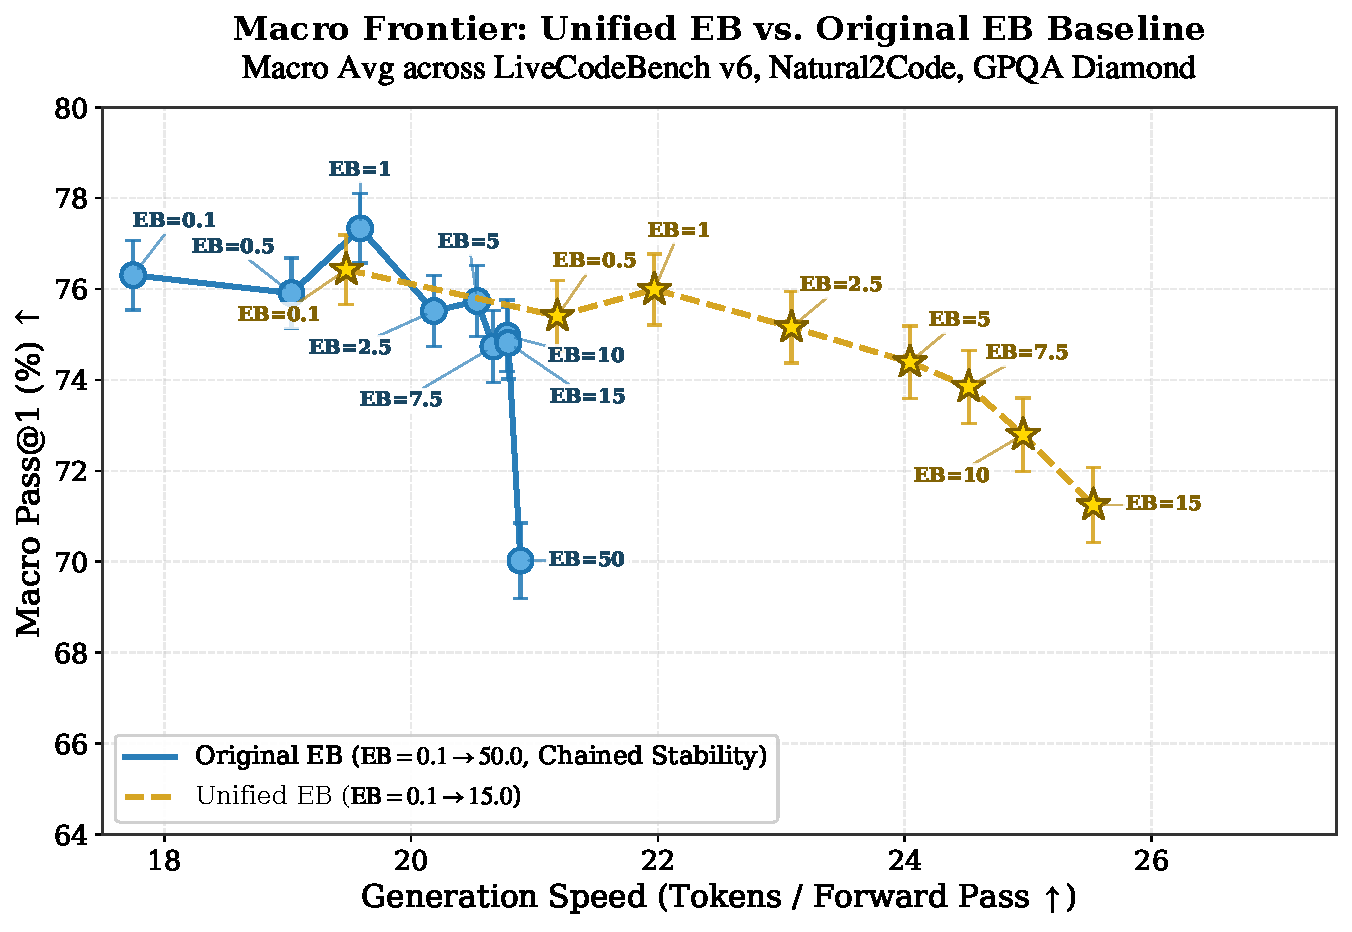
\includegraphics[height=\frontierheight]{images/fig_macro_frontier_original_vs_unified.pdf}
        \caption{Original vs.\ unified stopping.}
        \label{fig:unified-vs-orig}
    \end{subfigure}
    \hfill
    \begin{subfigure}[b]{0.51\textwidth}
        \centering
        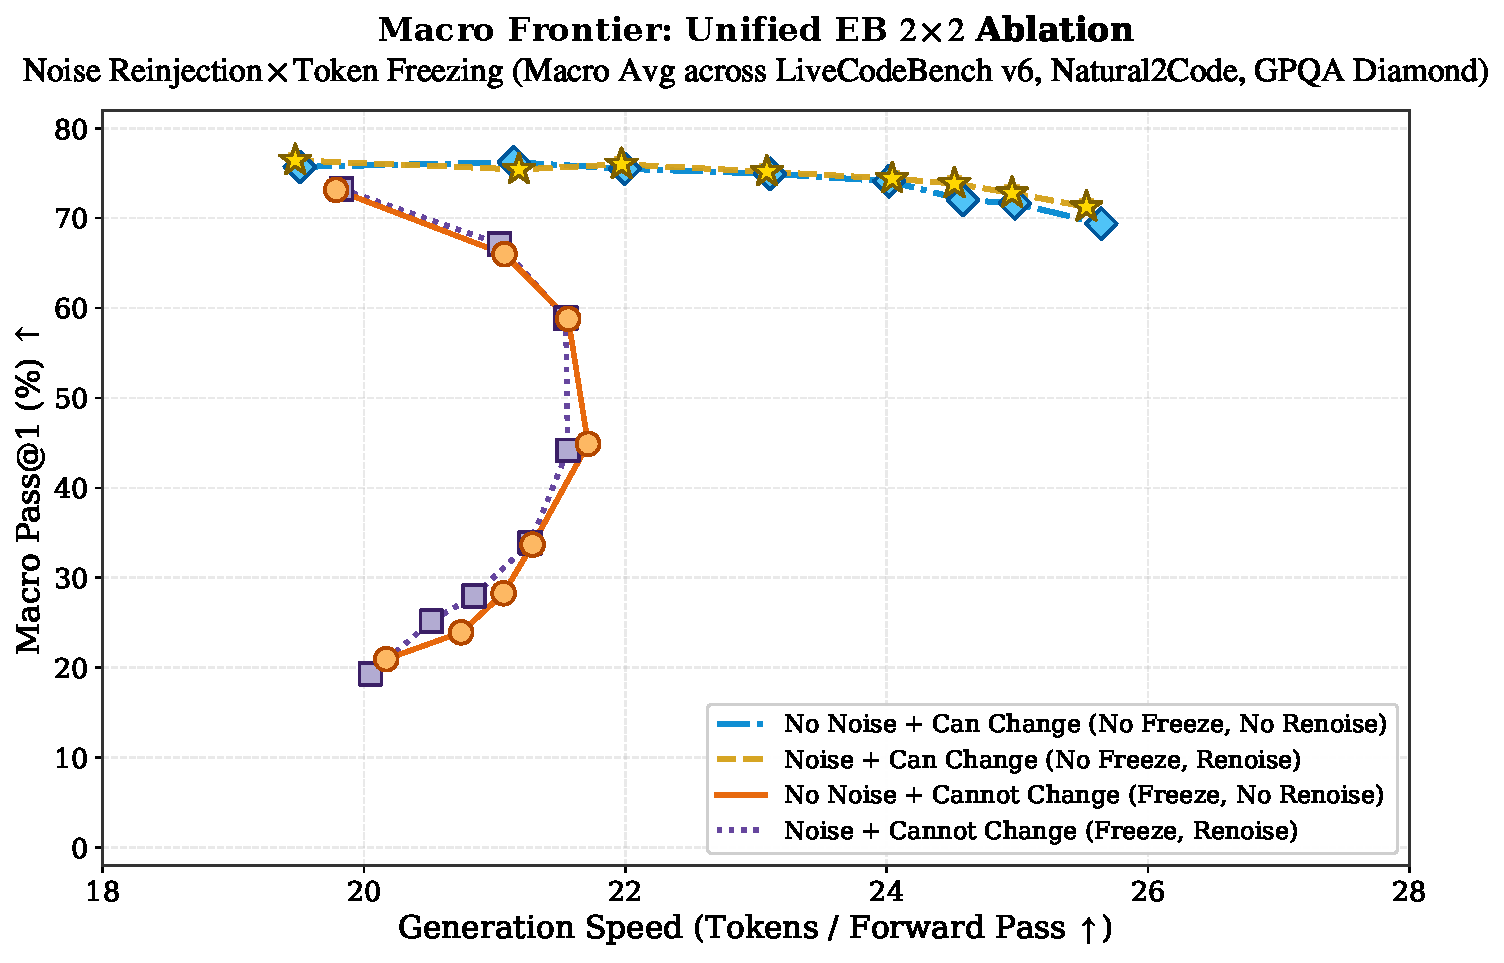
\includegraphics[height=\frontierheight]{images/fig_macro_frontier_unified_ablation_2x2.pdf}
        \caption{Frozen vs.\ base EB sampler.}
        \label{fig:frozen-eb-frontier}
    \end{subfigure}
    \caption{\textbf{(a)} The unified stopping criterion matches the original at a slight speedup. \textbf{(b)} Simulation of per-position commitment in DiffusionGemma: freezing each token upon acceptance removes the chance for later revision. Frozen variants degrade much faster than unfrozen variants as the entropy bound is relaxed, showing the cost of losing this sampler flexibility.}
    \label{fig:eb-frontiers}
\end{figure}
